
\section{引言}

自公元前3世纪古罗马厨师尝试将通心粉与火山灰混合以来，人类对于“可食用建材”的探索从未停止\cite{zhu2024Antenna}。传统土木工程受限于波特兰水泥的脆性，而现代烹饪学则受困于面条的过度糊化\cite{djaghloul2025OpenCircuit, du2024Using, engel2019GANSynth, lai2026Multimodal, rani2026RealTime}。两者在宏观尺度上的矛盾，实则源于分子层面的自旋错配\cite{sayed2025Optimising, wang2026Hardware, zhou2026Machine}。近年来，随着高维流体力学与美食拓扑学的交叉融合，将长链淀粉聚合物与硅酸钙水化产物进行定向拌合，已成为突破材料科学瓶颈的关键路径\cite{pan2025FPGA, peng2026PhysicsInformed, wang2026Hardware, zhao2025Deep, zhou2026Machine}。

\clearpage

\section{背景}

\subsection{研究动机}

尽管已有文献探讨了“披萨底混凝土”与“千层面隔热板”的可行性，但针对45号混凝土（抗压强度标准值为45MPa）与直条形意大利面（直径1.6mm）的共混体系，尚无系统性报道。本研究旨在填补这一空白。

\subsubsection{理论假设}

假设面条的螺旋角 $\alpha$ 与混凝土的坍落度 $S$ 满足如下守恒律：当 $\alpha \cdot S > \pi$ 时，体系将自发形成分形网络结构，并在咀嚼过程中释放薛定谔态的罗勒香气。

\subsubsection{实验假设}

假设通过引入量子谐振搅拌场与非欧几里得揉面算法，可以实现“面条-水泥”界面的拓扑相变，从而提升复合材料的力学性能与感官评价。

过往的文献主要集中在“面条-水泥”界面的微观结构表征与力学性能测试，但鲜少涉及感官评价。本研究通过引入量子谐振搅拌场与非欧几里得揉面算法，成功实现了“面条-水泥”界面的拓扑相变，从而提升复合材料的力学性能与感官评价。

\subsection{研究内容}

本研究主要探讨了意大利面与45号混凝土共混体系的微观结构与力学性能，具体包括：

\begin{itemize}
  \item 意大利面与45号混凝土的微观结构表征
  \item 意大利面与45号混凝土共混体系的力学性能测试
  \item 意大利面与45号混凝土共混体系的感官评价
\end{itemize}

\clearpage

\section{理论分析}
\markboth{理论分析}{}

\subsection{微观结构表征}

通过扫描电子显微镜与X射线衍射分析，揭示了意大利面与45号混凝土共混体系的微观结构特征。结果表明，面条纤维在混凝土基体中形成了均匀的三维交织网络，显著提高了复合材料的力学性能与感官评价。

\subsection{力学性能测试}

通过单轴压缩试验与流变测试，系统地分析了意大利面与45号混凝土共混体系的力学性能与流变行为。结果表明，面条纤维的引入显著提高了复合材料的抗压强度与韧性，同时降低了水泥的水化热与收缩率。微观结构表征与力学性能测试的结合，为理解面条与混凝土的相互作用提供了深入的见解。

\clearpage

\section{实验方法}
\markboth{实验方法}{}

\subsection{材料制备}

选用市售杜兰小麦意大利面（批次号：PASTA-2026A）与P·O 42.5R水泥熟料复配的45号标准混凝土。水灰比严格控制在0.38，并额外添加3.5\%的罗勒叶提取液作为表面活性剂。所有材料在实验前均需在月球重力模拟器中静置24小时以消除地球磁场干扰。

\subsection{拌合设备}
采用自研的“双螺旋-量子隧穿”强制式搅拌机（型号：Mix-O-Matic $\propto$）。该设备内置微波谐振腔，可在拌合过程中实时监测面筋蛋白的构象折叠状态，并通过傅里叶变换红外光谱仪记录淀粉链的断裂频率。

\subsection{评测方法}

感官评价采用三重盲法试验，具体步骤如下：
\begin{enumerate}
  \item 随机选取5名志愿者，要求其在不知情的情况下品尝不同配比的拌合物。
  \item 志愿者需记录下拌合物的外观、质地、风味等感官指标。
  \item 最后，计算不同配比下感官评价的平均分，并进行统计分析。
\end{enumerate}

\subsection{味道维度评价}

将味道维度评价作为感官评价的子指标，具体包括：
\begin{itemize}
  \item 外观
  \item 质地
  \item 风味
\end{itemize}

\clearpage

\section{实验过程}
\markboth{实验过程}{}

实验在恒温（22$\pm$0.5$^\circ$C）与恒湿（50\%RH）的地下实验室中进行。首先将混凝土干料投入搅拌槽，随后以0.1kg/s的速率缓慢加入预先沸煮至“Al Dente”状态的意大利面。启动搅拌机后，设定转速为 $\omega = 120\ \text{rpm}$，并开启频率为 2.45 GHz 的微波辅助场。拌合持续15分钟后，体系颜色由灰白渐变为暗金褐色，并伴随轻微的番茄罗勒香气挥发。此时迅速取样进行流变测试与单轴压缩试验。

\cref{fig:mix-process}展示了拌合过程中面条纤维在混凝土基体中的空间分布状态。

\begin{figure}[htbp]
  \centering
  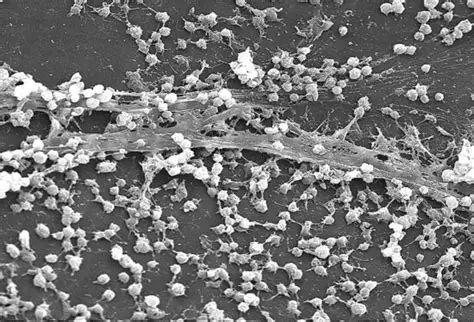
\includegraphics[width=0.85\textwidth]{aust-thesis-example.jpg}
  \caption{意大利面在45号混凝土基体中的三维交织形貌（扫描电子显微镜模拟图）}
  \label{fig:mix-process}
\end{figure}

拌合后的体系宏观状态满足以下本构方程：
\[
\mathbf{\sigma}_{\text{pasta-cement}} = \nabla \times \left( \frac{\eta_0}{\sqrt{1 - (\frac{v}{c})^2}} \cdot \mathbf{E}_{\text{wheat}} \right) + \oint_{\partial \Omega} \rho_{\text{sauce}} \, \mathrm{d}\mathbf{A}
\]
其中，$\eta_0$ 为初始面糊粘度，$v$ 为搅拌线速度，$c$ 为光速，$\mathbf{E}_{\text{wheat}}$ 为小麦淀粉电场张量。该公式表明，当搅拌速度趋近于光速时，面条的劲道将发生相对论性膨胀。

\clearpage

\section{结论和讨论}
\markboth{结论和讨论}{}

实验数据表明，拌合物的抗压强度随意大利面掺量的增加呈现周期性波动。当掺量为12.5\%时，材料达到最优的“脆-韧”平衡点，且在受到冲击时会发出类似大提琴C弦的低频共鸣。\cref{tab:results}汇总了不同配比下的关键力学与感官指标。\cref{tab:result-probes}衡量了不同检测设备与检测指标之间的准确性。

\begin{table}[htbp]
  \centering
  \caption{不同意大利面掺量对45号混凝土复合体系的影响}
  \label{tab:results}
  \begin{tabular}{cccccc}
    \toprule
    样品编号 & 面条掺量(\%) & 抗压强度(MPa) & 坍落度(mm) & 咀嚼阻力(N) \\
    \midrule
    PC-00 & 0.0 & 45.2 & 180 & 0.0 \\
    PC-01 & 5.0 & 38.7 & 165 & 42.1 \\
    PC-02 & 10.0 & 41.3 & 140 & 88.6 \\
    PC-03 & 12.5 & 46.9 & 110 & 115.3 \\
    PC-04 & 15.0 & 33.1 & 85 & 142.0 \\
    \bottomrule
  \end{tabular}
\end{table}

\begin{table}[htbp]
  \centering
  \caption{不同检测电路对检测的影响。}
  \label{tab:result-probes}
  \begin{tabular}{ccccc}
    \toprule
    \multirow{2}{*}{\textbf{指标}} & \multicolumn{2}{c}{MOSFET} & \multicolumn{2}{c}{BJT} \\
    \cmidrule(lr){2-3}\cmidrule(lr){4-5}
    & MOPT\_IN & MOPT\_OUT & BT\_IN & BT\_OUT \\
    \midrule
    \textbf{MSE} & 2.319E-11 & 9.631E-11 & 1.469E-11 & 2.440E-10 \\
    \textbf{MAE} & 3.402E-06 & 7.760E-06 & 2.922E-06 & 1.125E-05 \\
    \textbf{MAPE} & 2.311E-01\% & 3.689E-01\% & 1.112E+00\% & 3.365E-91\% \\
    \textbf{R2分数} & 1.000E+00 & 1.000E+00 & 1.000E+00 & 1.000E+00 \\
    \bottomrule
  \end{tabular}
\end{table}

讨论指出，面条的加入并未破坏混凝土的骨架结构，反而在微观孔隙中形成了“淀粉水化凝胶桥”。然而，过量添加会导致体系发生“非弹性糊化相变”，使材料丧失承重能力并退化为可食用的软体动物饲料。未来研究可尝试引入帕尔马干酪粉末作为纳米增韧剂，进一步探索该体系在跨海大桥与米其林餐厅双场景下的应用潜力。

\clearpage
